\documentclass[10pt,a4paper]{article}
\usepackage{rpgcover}
\usepackage{illustrated-panel}
\usepackage{longtable,booktabs}
\usepackage{float}
\usepackage{multicol}
\usepackage{fancyvrb}
\usepackage{wrapfig}
\usepackage{needspace}
\usepackage{titlesec}
\babelprovide[import]{ukrainian}
\titleformat{\subsection}{\normalfont\Large\bfseries\color{rpgbrown}}{}{0pt}{}
\titlespacing*{\subsection}{0pt}{12pt plus 2pt}{5pt}
\titleformat{\subsubsection}{\normalfont\normalsize\bfseries\color{rpgbrown}}{}{0pt}{}
\titlespacing*{\subsubsection}{0pt}{10pt plus 2pt}{4pt}
\usepackage{etoolbox}
% Stat boxes never start in the last lines of a page, where they would split after their title.
\BeforeBeginEnvironment{rpgnote}{\par\needspace{8\baselineskip}}
\pretocmd{\subsection}{\needspace{5\baselineskip}}{}{}
\pretocmd{\subsubsection}{\needspace{4\baselineskip}}{}{}
\setcounter{tocdepth}{1}
\clubpenalty=10000
\widowpenalty=10000
\displaywidowpenalty=10000
\interlinepenalty=0
\emergencystretch=1.2em
\newcommand{\HHInlineFigure}[3]{%
  \begin{center}\includegraphics[width=#2\linewidth,height=56mm,keepaspectratio]{assets/hollow-hearth/#1.jpg}%
  \par\vspace{2pt}{\footnotesize\itshape\color{rpgbrown}#3\par}\end{center}}
% Scene-opening illustrations float: here when they fit, otherwise at the foot of the next page.
% They never narrow a read-aloud box or leave a gap at the bottom of a page.
\newcommand{\HHSceneArt}[2]{%
  \begin{figure}[!hb]\centering\includegraphics[width=.62\linewidth,height=58mm,keepaspectratio]{assets/hollow-hearth/#1.jpg}%
  \par\vspace{2pt}{\footnotesize\itshape\color{rpgbrown}#2\par}\end{figure}}
% Full-page maps float to the next free page instead of ending the current page early.
\newcommand{\HHSceneMap}[3]{%
  \begin{figure}[p]\centering
    {\Large\bfseries\color{rpgbrown}#2\par}\vspace{6mm}%
    \includegraphics[width=.96\linewidth,height=190mm,keepaspectratio]{assets/hollow-hearth/#1.jpg}\par\vspace{4mm}%
    {\small\itshape\color{rpgbrown}#3\par}%
  \end{figure}}
\newcommand{\HHContents}{%
  \clearpage\thispagestyle{rpg}
  \vspace*{10mm}\begin{center}{\fontsize{27}{31}\selectfont\bfseries ЗМІСТ\par}\vspace{9pt}
  {\color{rpgline}\rule{.76\linewidth}{.55pt}}\end{center}\vspace{9mm}
  \begingroup
  \expandafter\def\csname l@section\endcsname##1##2{\csname @dottedtocline\endcsname{1}{0em}{4em}{\bfseries ##1}{##2}}%
  \csname @starttoc\endcsname{toc}\endgroup
  \vspace{5mm}
  \begin{center}
\includegraphics[height=68mm,width=.59\linewidth,keepaspectratio]{assets/hollow-hearth/front-overlay.png}\end{center}
  \vfill
  \begin{center}{\small\itshape Пригода Якопо Бішелли\par}\vspace{5pt}
  {\footnotesize Ця пригода, як і «Останній кидок», поширюється за ліцензією Creative Commons Attribution–ShareAlike 4.0 International (CC BY-SA 4.0). Дозволено поширювати й адаптувати її, також комерційно, за умови зазначення автора та збереження ліцензії у похідних творах.\par}\end{center}
  \clearpage}
\RPGSetRunningTitle{Дзвін Порожнього Вогнища}
\RPGSetCoverWordSpace{.78em}
\hypersetup{pdftitle={Дзвін Порожнього Вогнища},pdfauthor={Jacopo Biscella}}
\setlength{\emergencystretch}{2em}
\setcounter{secnumdepth}{-1}
\newcommand{\tightlist}{\setlength{\itemsep}{0pt}\setlength{\parskip}{0pt}}

\newcommand{\HHFrontArt}{assets/hollow-hearth/front-overlay.png}
\newcommand{\HHBackArt}{assets/hollow-hearth/back-overlay.png}
% Existing rpgcover.sty is used unchanged; only an adventure-specific back-cover layout follows.

\renewcommand{\RPGCoverTitleTypeface}{FreeSerif}
\renewcommand{\RPGCoverSubtitleTypeface}{FreeSerif}
\renewcommand{\RPGCoverTextTypeface}{FreeSerif}
\frenchspacing

\setlength{\parskip}{2.5pt plus .5pt minus .5pt}
\linespread{1.06}\selectfont
\newcommand{\HHAdventureBackCover}{%
 \clearpage\pagenumbering{gobble}\RPGCoverPagetrue\thispagestyle{empty}\null
 \begin{tikzpicture}[remember picture,overlay,x=1mm,y=1mm]
  \RPGDrawBackground{\RPGBackBackgroundFile}
  \node[align=center,text=coverink,text width=170mm,inner sep=0pt] at ($(current page.south west)+(105mm,260mm)$)
    {{\RPGCoverTitleFont\fontsize{19}{23}\selectfont ДЗВІН ПОРОЖНЬОГО ВОГНИЩА}};
  \draw[coverink,line width=.45pt] ($(current page.south west)+(57mm,246mm)$)--($(current page.south west)+(153mm,246mm)$);
  \node[anchor=north,align=left,text=coverink,text width=137mm,inner sep=0pt] at ($(current page.south west)+(105mm,240mm)$)
    {\RPGCoverTextFont\fontsize{10.4}{13.4}\selectfont
    Сім поколінь тому мандрівний Містик благословив бронзовий дзвін, відлитий у кузні маленького села там, де закінчується королівський шлях і починається старий ліс. Село назвали Порожнє Вогнище. Дзвін, у який били щосутінків, тримав Порожній Народ — блідих істот зі шкірою, мов кора, що шепочуть з-поміж дерев, — серед коренів.};
  \node[anchor=north,align=center,text=coverink,text width=140mm,inner sep=0pt] at ($(current page.south west)+(105mm,197mm)$)
    {\RPGCoverSubtitleFont\fontsize{13}{17}\selectfont Три ночі тому дзвін украли.\\[4pt]
    Наступна безмісячна ніч настане через сорок вісім годин.};
  \draw[coverink,line width=.45pt] ($(current page.south west)+(57mm,167mm)$)--($(current page.south west)+(153mm,167mm)$);
  \node[anchor=north,align=left,text=coverink,text width=137mm,inner sep=0pt] at ($(current page.south west)+(105mm,162mm)$)
    {\RPGCoverTextFont\fontsize{9.9}{12.1}\selectfont
    Вступна пригода для «Останнього кидка», для трьох або чотирьох Протагоністів на дві-три години. Вона навчає рівнів кидків, описових відстаней, запасу Ран, магії та Віддачі — і тієї миті, що дала грі назву.};
  \node[anchor=north,align=center,text=coverink,text width=147mm,inner sep=0pt] at ($(current page.south west)+(105mm,133mm)$)
    {\RPGCoverSubtitleFont\fontsize{10.5}{13.2}\selectfont
     Три підходи. Фінал обирає група.\\
     Зганьблений лицар. Покупець, що не той, ким здається.\\
     Рішення, яке група ухвалить разом.};
  \node[anchor=north,align=center,text=coverink,text width=144mm,inner sep=0pt] at ($(current page.south west)+(105mm,114mm)$)
    {\RPGCoverTextFont\fontsize{10.2}{12.5}\selectfont
     Містить: чотири мапи $\cdot$ п’ять ілюстрацій $\cdot$\\ коротку пам’ятку Оповідача з правилами й зустрічами.};
  \RPGOptionalArtwork{105}{59}{130}{24}{\HHBackArt}
  \filldraw[fill=white,draw=coverink,line width=.55pt]
    ($(current page.south west)+(139mm,25mm)$) rectangle
    ($(current page.south west)+(187mm,55mm)$);
 \end{tikzpicture}
 \clearpage\RPGCoverPagefalse
}
\newcommand{\HHFrontCover}{%
 \clearpage\RPGCoverPagetrue\thispagestyle{empty}\null
 \begin{tikzpicture}[remember picture,overlay,x=1mm,y=1mm]
  \RPGDrawBackground{\RPGFrontBackgroundFile}
  \node[align=center,text=coverink,text width=138mm,inner sep=0pt]
   at ($(current page.south west)+(105mm,248mm)$)
   {\RPGCoverTitleFont\fontsize{19}{23}\selectfont ДЗВІН\\[1.0mm]ПОРОЖНЬОГО ВОГНИЩА};
  \node[align=center,text=coverink,text width=135mm,inner sep=0pt]
   at ($(current page.south west)+(105mm,235mm)$)
   {\RPGCoverSubtitleFont\fontsize{9.0}{11.6}\selectfont Пригода для «Останнього кидка»};
  \RPGOptionalArtwork{105}{119}{150}{138}{\HHFrontArt}
  \node[align=center,text=coverink,text width=124mm,inner sep=0pt]
   at ($(current page.south west)+(105mm,25mm)$)
   {\RPGCoverTextFont\fontsize{12}{15}\selectfont Jacopo Biscella};
 \end{tikzpicture}\clearpage\RPGCoverPagefalse}
\begin{document}
% Select the language here: babel resets to its main language (english) at \begin{document}.
\selectlanguage{ukrainian}
\RPGStartFrontMatter
\HHFrontCover
\HHContents
\RPGStartMainMatter
\RPGChapter{Дзвін Порожнього Вогнища}
\begin{center}\textit{Вступна пригода для «Останнього кидка»}\par\smallskip
\small 2--3 години \textperiodcentered\ 3--4 Протагоністи \textperiodcentered\ Щонайменше один Боєць \textperiodcentered\ Видання для Оповідача
\end{center}
\noindent\textit{Чотири готові аркуші персонажів буде надано окремим PDF-файлом, по одному аркушу на Протагоніста, за шаблоном аркуша персонажа з книги правил.}\par\medskip
\subsection{Слово до Оповідача}\label{ux441ux43bux43eux432ux43e-ux434ux43e-ux43eux43fux43eux432ux456ux434ux430ux447ux430}

Ця пригода --- насамперед навчальний посібник і лише потім історія. Кожна сцена висуває на перший план одну з опор «\emph{Останнього кидка}», ніколи не зупиняючи оповідь заради лекції. Коли настане час фінальних титрів, гравці вже проживуть кидки за рівнями, описові відстані, спільний запас ОЗ для Ран і Втоми, механіку Допомоги та --- якщо ти добре впораєшся --- щонайменше одне Напруження, оголошене тремтячою рукою саме в ту мить, яку обіцяє назва гри.

Орієнтовний розклад:

\begin{itemize}
\tightlist
\item
  30 хвилин на створення персонажів і підготовку \emph{(скористайся правилами створення з посібника, с. 2--6)}
\item
  35 хвилин на \textbf{Сцену 1 · Село} (соціальне розслідування)
\item
  40 хвилин на \textbf{Сцену 2 · Шепітний ліс} (випробування вмінь + атмосфера)
\item
  60 хвилин на \textbf{Сцену 3 · Стару сторожову вежу} (кульмінаційний бій + розв’язка)
\item
  10 хвилин на \textbf{Три запитання} та наслідки
\end{itemize}

Нагадування, яке варто повторити: у цій грі немає кидків ініціативи, незмінного порядку ходів і клітинної сітки. Мапи, додані до пригоди, --- лише просторові орієнтири для уяви всіх за столом; відстані за столом завжди визначаються як \textbf{Впритул}, \textbf{Поруч}, \textbf{У межах досяжності} або \textbf{Далеко}.

\par\vspace{3pt}

\subsection{Чого навчає ця пригода}\label{ux447ux43eux433ux43e-ux43dux430ux432ux447ux430ux454-ux43fux440ux438ux433ux43eux434ux430}

\begingroup\setlength{\arrayrulewidth}{.34pt}\arrayrulecolor{rpgline}\renewcommand{\arraystretch}{1.32}\rowcolors{2}{rpgshade}{white}\par\smallskip\noindent\begin{tabularx}{\linewidth}{|Y|Y}\hline
\rpghead{Сцена} & \rpghead{Механіки, які вводяться} \\ \hline
Село & Кидки Характеристика + Вміння; ЦЗ для соціальних дій; протилежні кидки; залучення Риси й Тягаря \\ \hline
Шепітний ліс & Допомога; Стани ($-1$ щабель); описові категорії відстаней \\ \hline
Стара сторожова вежа & Бій; Рани й Втома; Критичний успіх; Віддача; \textbf{Напруження}; наслідки \\ \hline
\end{tabularx}\arrayrulecolor{black}\endgroup\par\smallskip

Якщо в групі є Містик, третя сцена, найімовірніше, стане місцем його першої Віддачі --- дозволь їй статися.

\par\vspace{3pt}

\par\needspace{65mm}\subsection{Передісторія}\label{ux43fux435ux440ux435ux434ux456ux441ux442ux43eux440ux456ux44f}

\begin{wrapfigure}{r}{.33\linewidth}\vspace{-8pt}\centering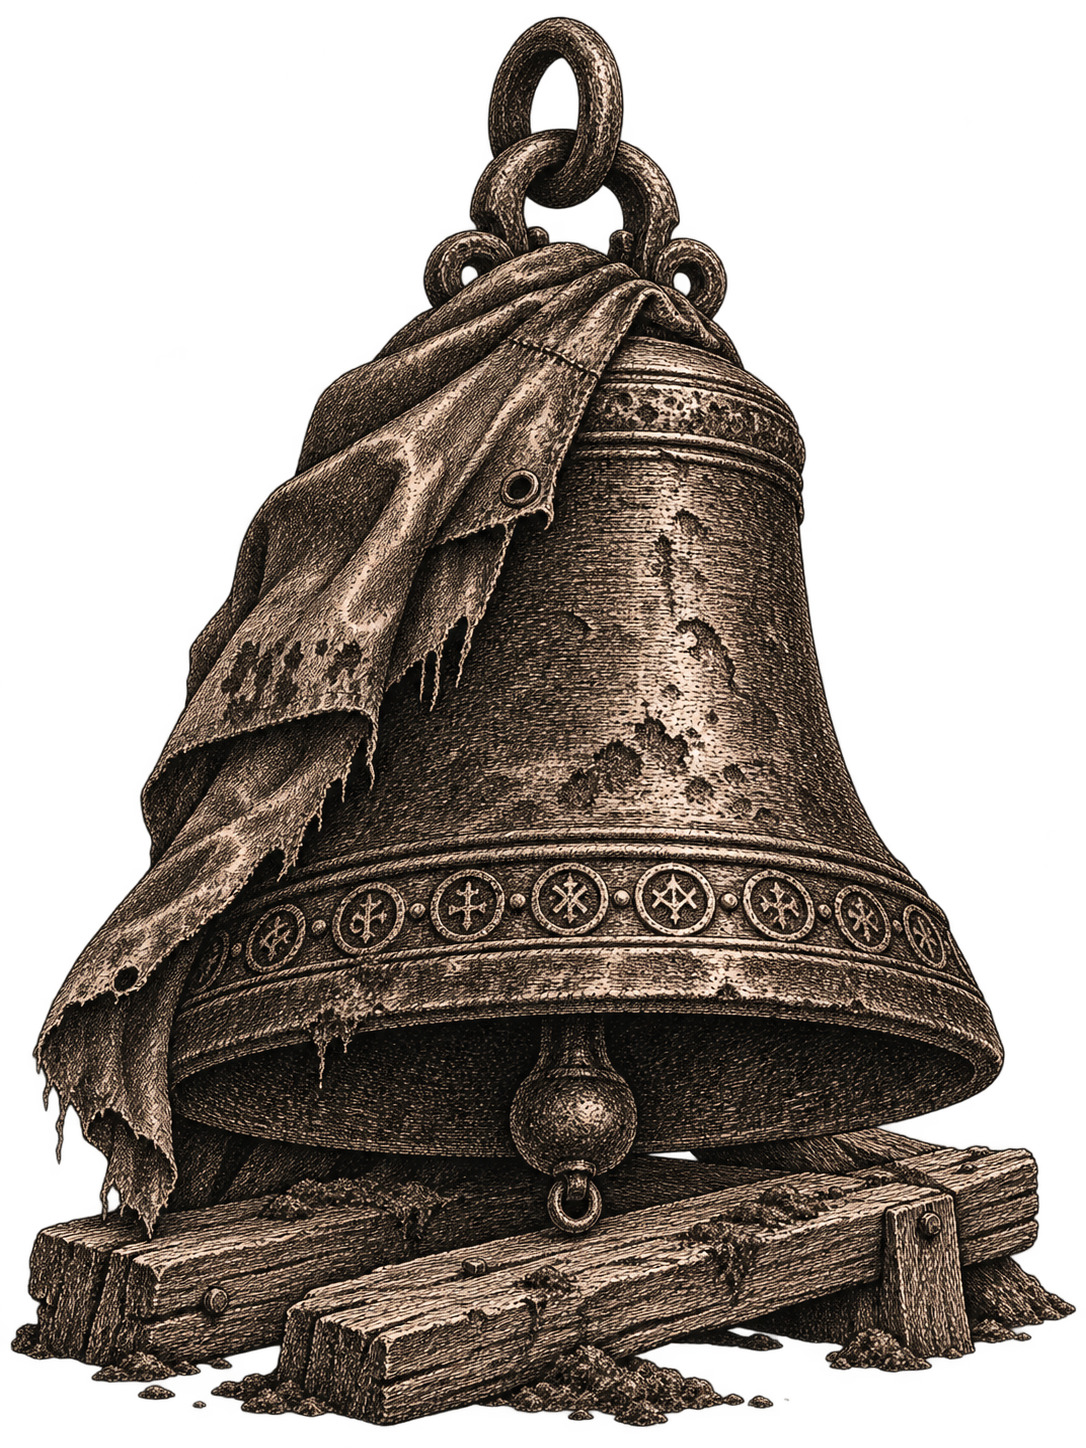
\includegraphics[width=.98\linewidth,height=52mm,keepaspectratio]{assets/hollow-hearth/bell.jpg}\par{\scriptsize\itshape\color{rpgbrown}Украдений дзвін, загорнутий у промаслене полотно}\vspace{-5pt}\end{wrapfigure}

Сім поколінь тому мандрівний Містик на ім’я \textbf{Вейл Ешен} благословив бронзовий дзвін, відлитий у кузні маленького поселення, збудованого там, де закінчується королівський шлях і починається стародавній ліс. Поселення назвали \textbf{Порожнє Вогнище}. Дзвін, у який били щосутінків, тримав \textbf{Порожній Народ} --- блідих істот зі шкірою, мов кора, що шепочуть з-поміж дерев, --- там, де йому й місце: серед коренів.

Три ночі тому дзвін украли.

Зграя розбійників на чолі з дезертиром, якого звуть \emph{«сер»} \textbf{Корвін Васк}, спустилася з руїн сторожової вежі, де вони таборують, убила учня старого дзвонаря й зникла на півночі в лісі, забравши дзвін, загорнутий у промаслене полотно. Учора вранці селяни поховали хлопця.

Наступна безмісячна ніч настане через \textbf{сорок вісім годин}.

Це і є відлік часу. Коли тієї ночі зайде місяць, а в сутінках не пролунає дзвін, Порожній Народ повернеться до Порожнього Вогнища, яке забуло, як себе захищати.

\par\vspace{3pt}

\subsection{Зачіпка}\label{ux43fux43eux447ux430ux442ux43eux43a-ux43fux440ux438ux433ux43eux434ux438}

\HHSceneArt{village}{Порожнє Вогнище в сутінках: порожній поміст}

Пристосуй прибуття героїв до Рис і Тягарів, які записали гравці. Кілька швидких підказок:

\begin{itemize}
\tightlist
\item
  \textbf{Учений}, що простежує родовід Вейла Ешена за старими літургійними записами.
\item
  \textbf{Авантюрист} з угодою від сусіднього містечка вище за шляхом.
\item
  \textbf{Містик}, який \emph{відчув}, як дзвін замовк, за багато миль звідси.
\item
  \textbf{Боєць}, що йде з поля бою, на якому більше не хоче бути.
\end{itemize}

Хоч яким шляхом вони прийдуть, сільська староста \textbf{Геста Траш} запропонує їм те небагато, що має Порожнє Вогнище, --- монети, гостинність і реліквію, збережену з часів заснування (див. \emph{Розв’язка}), --- щоб вони повернули дзвін додому.

\begin{quote}
\subsubsection{Прочитай уголос --- Прибуття}\label{ux43fux440ux43eux447ux438ux442ux430ux439-ux443ux433ux43eux43bux43eux441-ux43fux440ux438ux431ux443ux442ux442ux44f}

\emph{Шлях звужується до колії, колія --- до стежки, а стежка виводить на галявину з низькими кам’яними будинками під крутими шиферними дахами. Посеред сільського майдану стоїть дерев’яний поміст. Порожній. Чотири залізні болти там, звідки щось важке вирвали силою. З димарів не йде дим. На майдані --- ані душі.}

\emph{Потім відчиняються двері, виходить стара жінка, і за її спиною ви чуєте, як хтось плаче.}
\end{quote}

\par\vspace{3pt}

\HHSceneMap{map-village}{Порожнє Вогнище: план села}{Поміст для дзвона стоїть на майдані; Геста, Брам, Вела й заїзд --- неподалік. Усі місця в селі: Поруч.}
\RPGChapter{Сцена 1 --- Село}\label{ux441ux446ux435ux43dux430-1-ux441ux435ux43bux43e}

\textbf{Механічний акцент:} кидки Знання, бонуси Вмінь, протилежні кидки, залучення Риси й Тягаря.

У Порожньому Вогнищі є троє людей, важливих для вашого розслідування. Протагоністи можуть поговорити з усіма трьома в будь-якому порядку. Кожен тримає один фрагмент картини, і щонайменше один із них \emph{майже} бреше.

\par\smallskip\begin{rpgnote}[fontupper=\normalfont]\textbf{Персонажі села}\par\smallskip
\textbf{Геста Траш} \emph{(НІП)} --- Знання Компетентний. Бойових характеристик немає; якщо насильство торкнеться її, вона саме та, ким здається.\par\smallskip
\textbf{Вела Роан} \emph{(НІП)} --- Знання Експерт (Травництво, Виживання), Диво Компетентний. Не битиметься, якщо її не загнати в кут.\par\smallskip
\textbf{Старий Брам} \emph{(НІП)} --- Знання Компетентний. Битися вже не може.\end{rpgnote}\par\smallskip
Розташування показує \textbf{мапа села Порожнє Вогнище}. Усі місця в селі розташовані \textbf{Поруч} одне від одного.

\subsubsection{Геста Траш --- Староста}\label{ux433ux435ux441ux442ux430-ux442ux440ux430ux448-ux441ux442ux430ux440ux43eux441ux442ux430}

Жінка років шістдесяти, з обвітреним обличчям, висохла від горя. Її син пішов на війну й не повернувся; вона вже одинадцять років староста й знає кожного в селі на друге ім’я.

Що вона розповідає охоче:

\begin{itemize}
\tightlist
\item
  Розбійники прийшли зі \textbf{Старої сторожової вежі}, за чотири години ходьби на північ, у глибині Шепітного лісу.
\item
  Як останню нагороду від села вона пропонує реліквію часів заснування: \textbf{Соляний клинок} \emph{(посібник, с. 8)}.
\end{itemize}

Про що вона збреше:

Вона знає, що її двоюрідного брата \textbf{Маррела} бачили за випивкою з одним із розбійників у заїзді за тиждень до крадіжки. Вона не хоче, щоб брата за це повісили. \textbf{Кидок Знання, протилежний Знанню Гести (Компетентний)}, помічає її ніяковість. \textbf{Дипломатія} переконає її сказати правду; \textbf{Риторика} так само. \textbf{Залякування, ЦЗ 5}, теж спрацює, але до кінця пригоди село обернеться проти групи.

\begin{quote}
\subsubsection{Зачіпка для Риси й Тягаря}\label{ux437ux430ux447ux456ux43fux43aux430-ux434ux43bux44f-ux440ux438ux441ux438-ux439-ux442ux44fux433ux430ux440ux44f}

Протагоніст, чий Тягар пов’язаний із війною, утраченими дітьми чи порушеними клятвами, побачить у Гесті або союзницю, або дзеркало. Скористайся цим. \emph{«Ти нагадуєш мені його»}, --- каже вона, дивлячись не на ту людину.
\end{quote}

\subsubsection{Старий Брам --- Дзвонар}\label{ux441ux442ux430ux440ux438ux439-ux431ux440ux430ux43c-ux434ux437ux432ux43eux43dux430ux440}

Дзвонар, якому за вісімдесят, вижив лише тому, що, коли прийшли розбійники, справляв нужду в ожинових кущах. Убитий хлопець був його учнем і внучатим племінником. Брам розлючений. Не гучно. Інакше.

Що він бачив:

\begin{itemize}
\tightlist
\item
  Чотирьох чоловіків. Один в обладунку, один із довгим луком, двоє з кинджалами.
\item
  У того, що в обладунку, на плечі плаща було \textbf{вишито біле сонце} --- герб лицарського ордену, зганьбленого десять років тому. \textbf{Кидок Знання, ЦЗ 4, з Вмінням Історія} дозволяє впізнати \textbf{Орден Блідого Сонця}, розпущений за «ритуальні злочини» під час воєн. Без Історії --- \textbf{ЦЗ 5}, щоб видобути з пам’яті туманний спогад.
\item
  Він вірить, що дзвін живий. Можливо, він має рацію.
\end{itemize}

\subsubsection{Вела Роан --- Травниця}\label{ux432ux435ux43bux430-ux440ux43eux430ux43d-ux442ux440ux430ux432ux43dux438ux446ux44f}

Сорок років, гострий розум, єдина в селі, хто заходив \emph{углиб} Шепітного лісу й повернувся. Вона знає, що таке Порожній Народ. Прямо вона цього не скаже. Вона говорить оповідками.

Що вона запропонує, якщо правильно попросити:

\begin{itemize}
\tightlist
\item
  «Люди з кори» виходять із коренів, коли не дзвонить дзвін. Вона вірить, що один із Порожніх уже ходить серед селян у людській подобі.
\item
  Вона дасть флакон \textbf{дистильованого нічного кореня} --- \emph{визначний предмет: якщо полити ним лезо, наступний удар завдає +1 Рану неприродним створінням; лише одне застосування} --- \textbf{якщо} Протагоніст погодиться принести їй гілочку \textbf{місячносрібної квітки} з глибини лісу.
\end{itemize}

Це побічна спокуса: нагода для моменту Тягаря, якщо згодом хтось порушить слово, або нагода випробувати шляхетну Рису. Квітка існує. Чи знайде група на неї час --- вирішувати їй.

\subsubsection{Необов’язково · Маррел, двоюрідний брат}\label{ux434ux43eux434ux430ux442ux43aux43eux432ux43e-ux43cux430ux440ux440ux435ux43b-ux434ux432ux43eux44eux440ux456ux434ux43dux438ux439-ux431ux440ux430ux442}

Якщо Протагоністи розплутують брехню Гести, Маррела можна знайти в заїзді, де він заливає свій страх. Він підтверджує, що розбійник, з яким він говорив, --- чоловік на ім’я \textbf{Тессік} --- вихвалявся покупцем, який \emph{«платить північним сріблом»} і прийде по дзвін. Маррел не знав, що дзвін украдуть. \textbf{Залякування, ЦЗ 4}, зламає його. \textbf{Дипломатія, ЦЗ 4}, за чаркою теж спрацює. \textbf{Торгівля, ЦЗ 4}, якщо Учений захоче розібратися, що насправді означає «північне срібло» (так кажуть контрабандисти, які перетинають кордон: північного срібла не існує, це умовна назва золота фей).

\subsubsection{Порада для Оповідача}\label{ux43fux43eux440ux430ux434ux430-ux43eux43fux43eux432ux456ux434ux430ux447ux435ux432ux456}

Коли гравець заявляє \emph{«Хочу зрозуміти, чи вона бреше»}, запитай \textbf{як}. Тисне? Спостерігає? Ловить її на суперечності? Саме \emph{як} визначає Характеристику й Вміння. \textbf{Знання} --- типовий вибір, щоб читати людину; \textbf{Етикет} ловить її на придворних обмовках, \textbf{Залякування} змушує помилятися, \textbf{Обман} дає змогу перебрехати її й загнати в кут. Окремої підсистеми соціального бою немає. Є лише Знання плюс доречне Вміння проти ЦЗ. Як і в усьому іншому.

\par\vspace{3pt}

\HHSceneMap{map-forest}{Крізь Шепітний ліс}{Село внизу, вежа вгорі; Порожній Народ з’являється на березі, який група щойно залишила.}

\RPGChapter{Сцена 2 --- Шепітний ліс}\label{ux441ux446ux435ux43dux430-2-ux448ux435ux43fux456ux442ux43dux438ux439-ux43bux456ux441}

\HHSceneArt{hollow}{Спостерігач серед дерев}

\textbf{Механічний акцент:} механіка Допомоги, категорії відстаней, Стани як $-1$ щабель.

Від села на північ веде стежка з прим’ятої папороті й загублених клаптиків промасленого полотна. За п’ятдесят кроків Шепітний ліс поглинає її. Дерева тут нахиляються досередини.

\begin{quote}
\subsubsection{Прочитай уголос --- Вхід до лісу}\label{ux43fux440ux43eux447ux438ux442ux430ux439-ux443ux433ux43eux43bux43eux441-ux443-ux43bux456ux441ux456}

\emph{Щойно ви перетинаєте узлісся, світла стає на третину менше. Не через крони --- крон, гідних так називатися, тут немає, --- а ніби саме повітря його випиває. Звуки глухнуть. Кроки перестають відлунювати. Після десяти хвилин ходьби ви чуєте лише власне дихання й десь дуже далеко щось, що може бути вітром у гіллі, а може --- голосами, які кажуть щось, чого ви ніяк не розберете.}
\end{quote}

Шлях від села до сторожової вежі показує \textbf{мапа подорожі Шепітним лісом}; на ній позначено міст і місце Появи.

\subsubsection{Стежка · Випробування Виживання}\label{ux441ux442ux435ux436ux43aux430-ux432ux438ux43fux440ux43eux431ux443ux432ux430ux43dux43dux44f-ux432ux438ux436ux438ux432ux430ux43dux43dux44f}

Слід справжній, але його легко загубити. Персонаж із Вмінням \textbf{Виживання} кидає \textbf{Спритність, ЦЗ 4}. Персонаж зі Спритністю на рівні Компетентний і з цим Вмінням кидає 2d6 і бере більший; Експерт у Спритності без Вміння кидає так само; Недосвідчений у Спритності без Вміння кидає 2d6 і бере менший, що жорстоко.

Це ідеальна мить, щоб познайомити гравців із \textbf{Допомогою} \emph{(посібник, с. 7)}:

\begin{itemize}
\tightlist
\item
  \textbf{Компетентний помічник} --- той, чий власний кидок у цьому ж випробуванні був би на рівні Експерт або вище, --- додає \textbf{+1d6} до набору кубиків основного персонажа без жодного штрафу.
\item
  \textbf{Некомпетентний помічник} --- будь-хто, хто в цьому ж випробуванні кидав би нижче рівня Експерт, --- додає \textbf{+1d6}, \emph{але підвищує ЦЗ на 1}. Боєць, який гучно «допомагає» Авантюристу шукати сліди, може тільки погіршити справу.
\end{itemize}

Нехай гравці побачать це на власні очі. Боєць, що допомагає слідопиту, перетворює ЦЗ 4 на ЦЗ 5 --- і засвоює урок, коли слід загублено.

Якщо слід загублено, минає зайва година, і сутінки застають групу в лісі. Відтоді й до світанку всі кидки робляться під \textbf{Станом: $-1$ щабель}.

\subsubsection{Гнилий міст}\label{ux433ux43dux438ux43bux438ux439-ux43cux456ux441ux442}

Стежка перетинає ущелину по мосту з однієї колоди, який не лагодили двадцять років. Колода витримає лише одну людину за раз. Унизу, за п’ятнадцять метрів, струмок біжить по камінню.

\begin{itemize}
\tightlist
\item
  \textbf{Кидок Спритності, ЦЗ 4}, щоб безпечно перейти. З \textbf{Акробатикою} --- без жодних труднощів.
\item
  Персонаж, який падає, отримує \textbf{2 Рани} (бойові --- від каміння). \textbf{Кидок Медицини, ЦЗ 4}, у межах сцени відновлює 1 Рану (2 у разі Критичного успіху).
\item
  Мотузка, натягнута як поруччя (\textbf{Сила + Ремесла або + Витривалість, ЦЗ 3}), знижує ЦЗ для всіх до 3 і скасовує наслідки провалу.
\end{itemize}

Це також тиха перевірка Риси. Протагоніст із Рисою \emph{«Я нікого не покидаю»}, який провалить власний кидок переходу, а потім його переведе товариш, має це відчути.

\subsubsection{Поява}\label{ux43fux43eux44fux432ux430}

Хоч би як група перебралася --- вдало чи погано, --- щойно \textbf{остання людина ступає на протилежний бік}, між двома деревами на щойно покинутому боці з’являється \textbf{один із Порожніх}. Блідий. Зі шкірою, мов кора. Трохи зависокий. Рот не зовсім там, де мав би бути рот. Він не рухається. Не погрожує. Він дивиться, як вони відходять. Через тридцять секунд його вже немає.

Це лише атмосфера. Кидка немає. Дай гравцям побути з цим.

\begin{quote}
\subsubsection{Порада --- Відстані}\label{ux43fux43eux440ux430ux434ux430-ux432ux456ux434ux441ux442ux430ux43dux456}

Порожній --- \textbf{Далеко} (по той бік ущелини, поза розумною дальністю пострілу з лука). Містик із Гримуаром сприйняття --- наприклад, \emph{Оком порожнечі} (посібник, с. 10) --- може захотіти роздивитися ближче. Дозволь. Нехай сплатить ціну Втомою. Покажи столу, як виглядає кидок Дива, коли на кону лише знання.
\end{quote}

\subsubsection{Вовки · Необов’язкова сутичка для балансу}\label{ux432ux43eux432ux43aux438-ux43dux435ux43eux431ux43eux432ux44fux437ux43aux43eux432ux430-ux441ux443ux442ux438ux447ux43aux430}

Якщо гра йде швидко, а групі явно бракує випробувань, пара \textbf{голодних вовків} може напасти з засідки на останньому відрізку перед вежею. Два вовки навчають правила \textbf{ворожих груп} (посібник, с. 12) і дають Бійцю вперше змахнути зброєю. \par\smallskip\begin{rpgnote}[fontupper=\normalfont]\textbf{Голодний вовк} \emph{(необов’язкова сутичка в лісі)} \emph{ЦЗ: С3/Спр4 · Компетентний · 2 Рани · укус (2Р від Сили).} \emph{Поведінка: «Полює на найслабшого. Три ночі без їжі».}\end{rpgnote}

\par\vspace{3pt}

\RPGChapter{Сцена 3 --- Стара сторожова вежа}\label{ux441ux446ux435ux43dux430-3-ux441ux442ux430ux440ux430-ux441ux442ux43eux440ux43eux436ux43eux432ux430-ux432ux435ux436ux430}

\HHSceneArt{tower}{Стара сторожова вежа в сутінках}

\textbf{Механічний акцент:} бій як розмова, Рани й Втома, Критичний успіх, Віддача, \textbf{Напруження}.

Стара сторожова вежа --- два поверхи щербатого каменю на невисокому пагорбі; половини даху немає, у тріщинах плющ. Перед входом жевріє багаття. Біля нього сидять двоє розбійників. На нижньому поверсі сплять ще двоє. На верхньому поверсі \textbf{сер Корвін Васк} сидить поруч із дзвоном, загорнутим у промаслене полотно, і чекає покупця.

Покупець має прийти \textbf{опівночі}. Зараз сутінки.

Нижній поверх і підходи до вежі показує \textbf{мапа нижнього поверху Старої сторожової вежі}, а планування верхнього поверху, де відбувається кульмінація, --- \textbf{мапа верхнього поверху Старої сторожової вежі}.
\HHInlineFigure{map-ground}{.68}{Стара сторожова вежа: нижній поверх --- вхід і багаття на півдні, обвалена стіна на заході, сходи на півночі.}

\par\smallskip\begin{rpgnote}[fontupper=\normalfont]\textbf{Розбійники}\par\smallskip \textbf{Розбійник} \emph{ЦЗ: С3/Спр3 · Компетентний · 2 Рани · кинджал (2Р від Спритності) або короткий кийок (1В від Сили).} \emph{Поведінка: «Боягузи в чесному бою. Тікають, якщо Корвін падає».} \emph{Як група: один кидок, +1Р за кожного учасника понад першого (максимум +3). Кожна Рана, завдана групі, усуває одного її члена.}\end{rpgnote}\par\smallskip
\subsubsection{Три підходи}\label{ux442ux440ux438-ux43fux456ux434ux445ux43eux434ux438}

У групи є варіанти. Перед будь-якими кидками просто запитай: \emph{«Як ви хочете це зробити?»} Механіки змінюються відповідно.

\textbf{Потайність.} Обвалену стіну із західного боку можна помітити \textbf{кидком Знання + Тактика, ЦЗ 3}, або просто з опису. Кожен персонаж кидає \textbf{Спритність + Потайність, ЦЗ 4}, щоб підійти непоміченим. Один провал насторожує двох розбійників біля багаття. Два провали піднімають усіх, зокрема й Корвіна. Чистий підхід дає групі змогу дістатися верхнього поверху й захопити його зненацька.

\par\Needspace{10\baselineskip}\noindent\textbf{Перемови.} Підійти до багаття й заговорити. Корвін --- людина зі зламаною гордістю. Якщо Протагоніст (особливо Боєць) звернеться до нього \emph{«сер Корвін»}, його Тягар дасть тріщину. \textbf{Знання + Дипломатія або Риторика, ЦЗ 5}, переконає його \emph{подумати} про те, щоб продати дзвін назад, а не покупцю. Він вимагатиме більше, ніж нагорода села, --- але група може це пообіцяти. Збрехати йому про нагороду --- це \textbf{кидок Знання + Обман, протилежний його Знанню (Компетентний)}.

\textbf{Штурм.} Увірватися з боєм. Двоє розбійників біля багаття, двоє всередині, Корвін нагорі. Гучно, криваво --- і найпростіший спосіб навчити новачків бою.

\par\smallskip\begin{rpgnote}[fontupper=\normalfont]\textbf{Сер Корвін Васк, зганьблений лицар} \emph{ЦЗ: С4/Спр5 · Експерт · 6 Ран · довгий меч (2Р від Сили) · важкий обладунок.} \emph{Поведінка: «Не вдарить людину, що стоїть навколішки. Прийме двобій від будь-кого, хто назве його “сер”. Ненавидить Містиків --- так його навчив орден».} \emph{Необов’язково: він носить пошарпаний медальйон із портретом сестри всередині. Якщо Протагоніст побачить його під час бою, дай йому нагоду цим скористатися.}\end{rpgnote}\par\smallskip
\subsubsection{Верхній поверх}\label{ux432ux435ux440ux445ux43dux456ux439-ux43fux43eux432ux435ux440ux445}

Дзвін, сер Корвін і кульмінаційне зіткнення --- усе це на верхньому поверсі. Його планування важливе, бо від нього залежать тактичні рішення гравців.

\par\medskip\noindent
\begin{tabular}{@{}p{.60\linewidth}@{\hspace{.028\linewidth}}p{.345\linewidth}@{}}
\centering\vspace{0pt}
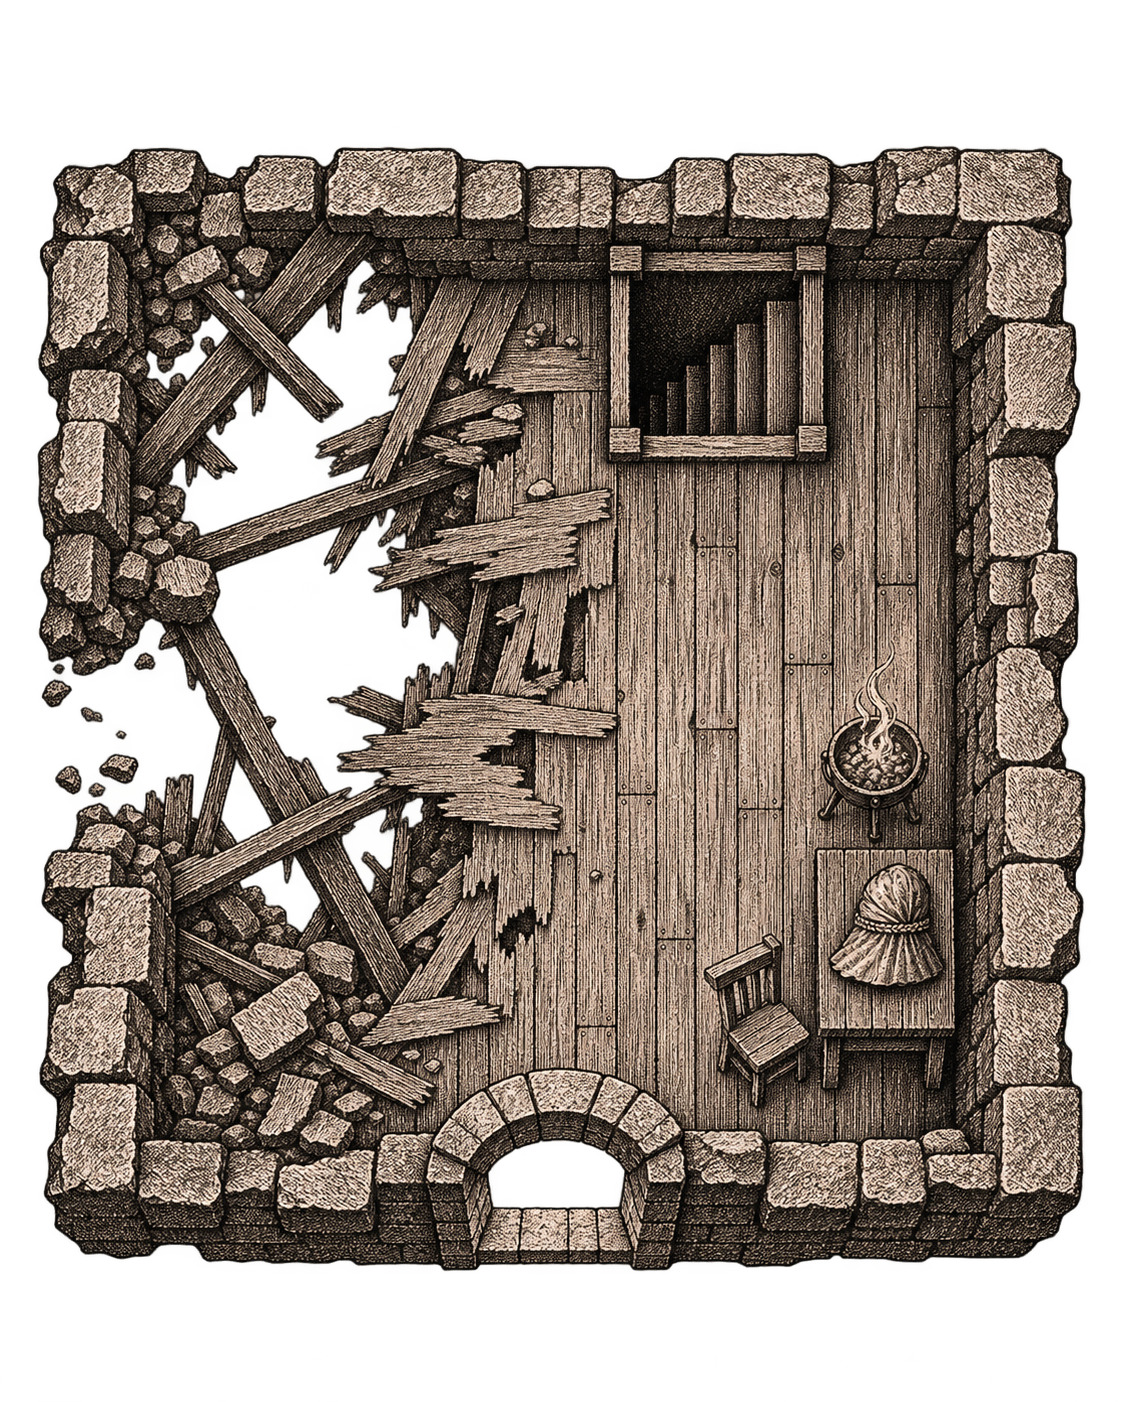
\includegraphics[width=.98\linewidth,height=70mm,keepaspectratio]{assets/hollow-hearth/map-upper.jpg}\par\vspace{2pt}
{\footnotesize\itshape\color{rpgbrown}Стара сторожова вежа: верхній поверх\par}
{\scriptsize Північні сходи; відкритий західний бік; південне вікно, дзвін і жаровня в уцілілій східній частині.\par}
&
\centering\vspace{0pt}
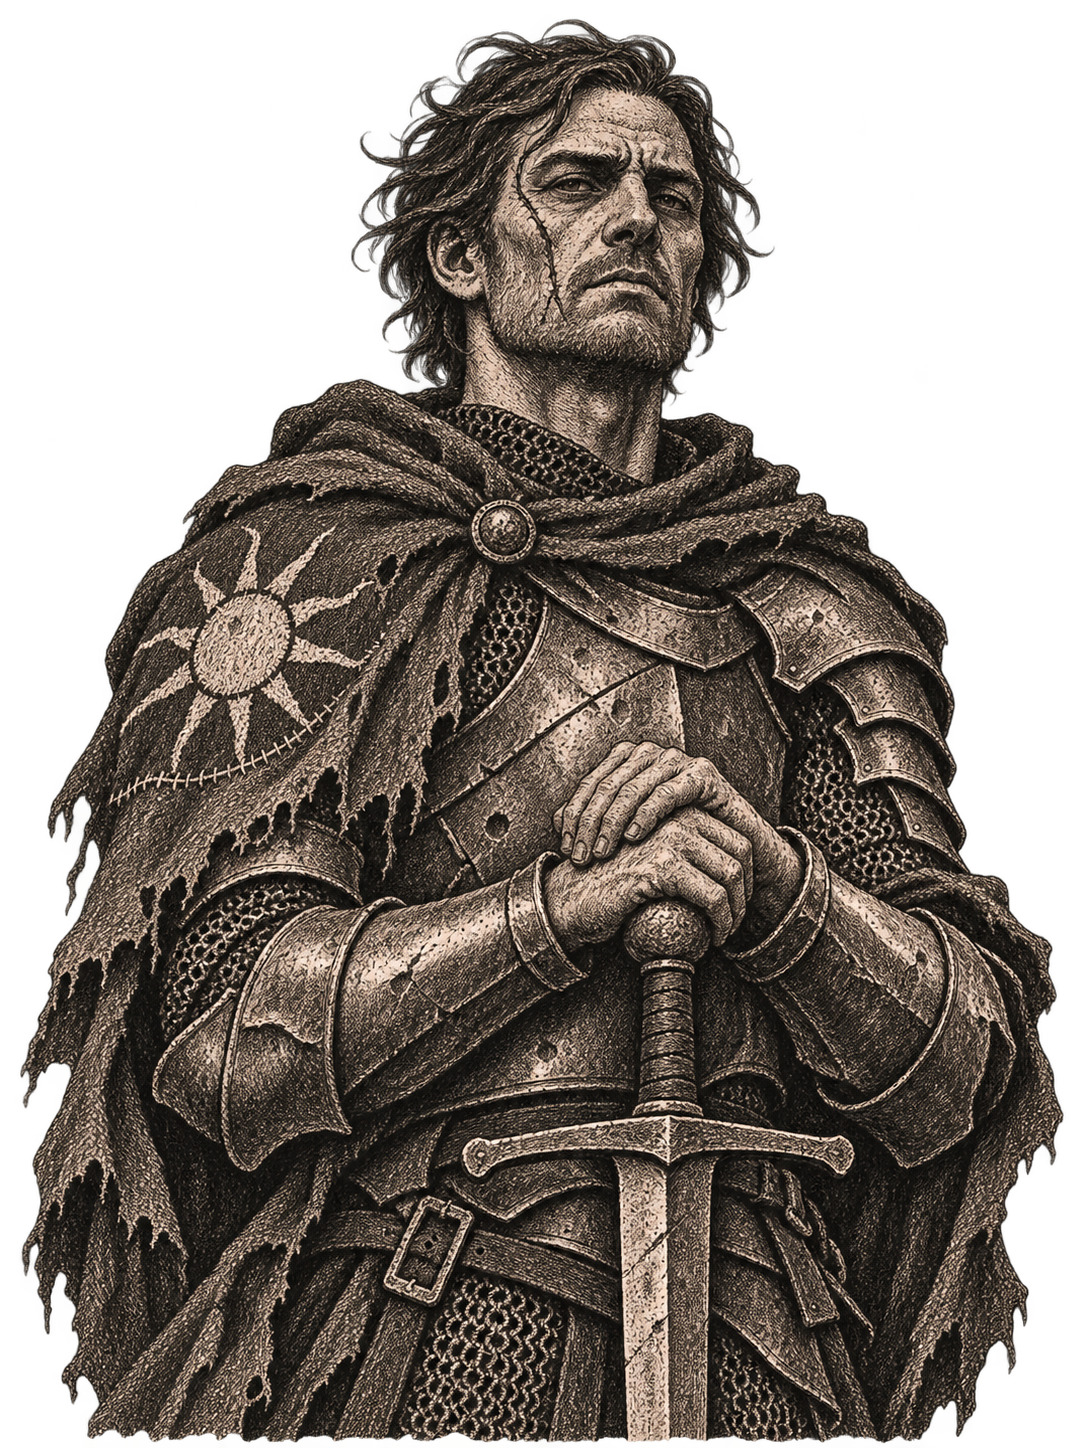
\includegraphics[width=.95\linewidth,height=68mm,keepaspectratio]{assets/hollow-hearth/corwin.jpg}\par\vspace{2pt}
{\footnotesize\itshape\color{rpgbrown}Сер Корвін Васк\par}
\end{tabular}
\par\medskip

Сер Корвін сидить на дерев’яному стільці біля \textbf{південного вікна} й стежить за стежкою, якою прийде покупець. Дзвін стоїть поруч на столику, досі загорнутий у забруднене промаслене полотно. Жаровня з тліючим вугіллям --- єдине тепле світло в кімнаті. Сходи виходять нагору біля північної стіни --- \textbf{за його спиною}.

\textbf{Над західною половиною верхнього поверху --- відкрите небо}: той самий обвал, що зруйнував західну стіну на нижньому поверсі, забрав західну частину даху й частину західного настилу. Розхитані балки звисають навскіс. Відкритим західним настилом небезпечно ходити без обережності.

Це створює \textbf{четвертий підхід}, на який текст вище лише натякав:

\textbf{Підйом.} Персонаж з \textbf{Акробатикою} може видертися на купу уламків обваленої стіни на нижньому поверсі, піднятися далі зовнішнім боком зруйнованої західної стіни й проникнути всередину через пролом у даху. Кидок \textbf{Спритність + Акробатика, ЦЗ 4}, щоб видертися чисто; без Акробатики --- \textbf{ЦЗ 5}. Провал означає падіння --- 1 Рана від висоти плюс шум падіння (Корвін почує). У разі успіху персонаж зістрибує на верхній поверх \emph{за спиною} Корвіна й захоплює його зненацька. Цей підхід --- лише для одного персонажа: Боєць у важкому обладунку не зможе так видертися, а Містик із 2 ОЗ не може дозволити собі падіння в разі провалу. \textbf{Найкраще для цього підходить спритний Авантюрист.}

\par\Needspace{12\baselineskip}\noindent\textbf{Тактичні особливості верхнього поверху:}

\begin{itemize}
\tightlist
\item
  \textbf{Південне вікно.} Той, хто дістанеться дзвона, може викинути його назовні --- він важко впаде біля багаття внизу й, можливо, трісне. Покупець, що спостерігає зі стежки, це побачить. Протагоніст може також утекти з кімнати через вікно, зістрибнувши на землю (Спритність + Акробатика, \textbf{ЦЗ 4}, щоб приземлитися чисто; провал коштує 1 Рану).
\item
  \textbf{Небезпечна західна половина.} Бій на обваленій половині ведеться під Станом: \textbf{$-1$ щабель}. Персонаж, якого скинули за край, падає на один поверх (2 Рани). Корвін, який знає кімнату, битиметься лише на східній половині --- і охоче спробує зіштовхнути ворогів на хиткий настил.
\item
  \textbf{Жаровня.} Якщо її перекинути, жар розсиплеться по сухій дерев’яній підлозі --- вогонь пошириться за дві сцени дії, і в кімнаті неможливо буде перебувати. Відчайдушний хід, доступний будь-кому, що може врятувати групу або знищити дзвін разом з усім іншим.
\item
  \textbf{Важкий обладунок сера Корвіна.} Його важкий обладунок встановлює ЦЗ, щоб влучити в нього, на рівні \textbf{4 для Сили} або \textbf{5 для Спритності}. Шкоди він не зменшує. Перекинута жаровня, поштовх до обваленого краю чи Критичний успіх Протагоніста, який оголосив Напруження, можуть змінити хід зіткнення.
\end{itemize}

\subsubsection{Масштабування сутички}\label{ux441ux43aux43bux430ux434ux43dux456ux441ux442ux44c-ux441ux443ux442ux438ux447ux43aux438}

\begingroup\setlength{\arrayrulewidth}{.34pt}\arrayrulecolor{rpgline}\renewcommand{\arraystretch}{1.32}\rowcolors{2}{rpgshade}{white}\par\smallskip\noindent\begin{tabularx}{\linewidth}{|Y|Y|Y}\hline
\rpghead{Розмір групи} & \rpghead{Розбійники} & \rpghead{Сер Корвін} \\ \hline
3 гравці & 3 розбійники (група) & Так \\ \hline
4 гравці & 4 розбійники (2 зовні, 2 всередині) & Так \\ \hline
\end{tabularx}\arrayrulecolor{black}\endgroup\par\smallskip

Якщо групі, схоже, дуже важко, нехай один розбійник утече за першої ознаки справжнього кровопролиття. Якщо вона проходить усе без зусиль, покупець приходить раніше.

\subsubsection{Поворот · Покупець}\label{ux43fux43eux432ux43eux440ux43eux442-ux43fux43eux43aux443ux43fux435ux446ux44c}

Якщо група все ще біля вежі \textbf{опівночі} --- посеред бою, перемов чи вже перемігши, --- з лісу виходить одинока постать у балахоні, без обличчя під каптуром. \textbf{Покупець --- один із Порожніх у людській подобі.} Він хоче, щоб дзвін замовк назавжди, а не був знищений. У нього невеликий мішечок срібла. Він говорить тими самими не зовсім правильними голосами, які група ледь розчула, коли входила до лісу.

\par\smallskip\begin{rpgnote}[fontupper=\normalfont]\textbf{Покупець (Порожній у людській подобі)} \emph{ЦЗ: С3/Спр4 · Експерт · 4 Рани · дотик (1В від Дива; у разі Критичного успіху 2Р + Стан до кінця сцени) · без обладунку.} \emph{Поведінка: «Вимовляє не ті склади. Дерева не відповідають. Замість крові сочиться сік».}\end{rpgnote}\par\smallskip
Це \textbf{момент вибору}. Група може:

\begin{itemize}
\tightlist
\item
  \textbf{Відмовитися й битися.} \emph{(Характеристики вище.)}
\item
  \textbf{Узяти срібло.} Група йде багатою. Порожнє Вогнище більше ніхто не побачить живим. \emph{Якщо гравці це оберуть, нехай це буде справжній фінал.}
\item
  \textbf{Збрехати й улаштувати покупцю засідку.} Протилежні \textbf{кидки Знання проти Знання покупця (Експерт)}. Якщо група перемагає, вона залишає собі і срібло, \emph{і} дзвін, --- але ліс позначив їх, і наступна пригода почнеться з цієї мітки.
\end{itemize}

\subsubsection{Кульмінація --- і останній кидок}\label{ux43aux443ux43bux44cux43cux456ux43dux430ux446ux456ux44f-ux43eux441ux442ux430ux43dux43dux456ux439-ux43aux438ux434ux43eux43a}

Хоч який шлях оберуть гравці, кульмінація має залишити щонайменше одного Протагоніста в стані \textbf{Побитий} або \textbf{Важкий}. Стеж за ОЗ за столом. Щойно гравець опускається до \textbf{1 ОЗ}, а йому ще треба зробити кидок, щоб завершити сцену, --- зупинися. Подивися на нього через стіл. Запитай:

\begin{quote}
\emph{«Це останній кидок. Готовий заплатити за нього кров’ю?»}
\end{quote}

Проведи гравця через оголошення \textbf{Напруження} \emph{(посібник, с. 13)}. Нехай кидає; Рана Втоми настає після кидка. \textbf{Це та мить, на честь якої названо гру.} Нехай вона так і відчувається. Якщо кидок вдасться, за столом мають радіти. Якщо ні --- за столом має запасти тиша.

\par\vspace{3pt}

\subsection{Розв’язка}\label{ux440ux43eux437ux432ux44fux437ux43aux430}

Три чисті завершення з наслідками, що дають зерно для наступної пригоди:

\textbf{Дзвін повертається.} Геста вручає \textbf{Соляний клинок} і всю гостинність села. Якщо Велі принесли квітку, вона вважає групу своїми друзями. Чутки доходять до сусіднього містечка. \emph{Наступна пригода починається з того, що героїв розшукують на ім’я.}

\textbf{Дзвін змушено замовкнути або продано.} Група йде багатою й позначеною. Порожній Народ запам’ятовує їх. \emph{Одна з майбутніх пригод почнеться з нічного шепоту, що знає їхні імена.}

\textbf{Дзвін знищено.} Чи через невдалу Віддачу, чи через відчайдушний бій --- у безмісячну ніч Порожній Народ повертається до Порожнього Вогнища. \emph{Наступна пригода починається зі спроби все виправити. Вейл Ешен, той самий перший Містик, можливо, не такий уже й мертвий, як кажуть хроніки.}

\subsubsection{Три запитання}\label{ux442ux440ux438-ux437ux430ux43fux438ux442ux430ux43dux43dux44f}

Заверши сесію тим, що група разом відповідає на три запитання Розвитку (посібник, с. 11). Правильна оцінка --- чесна, а не щедра. Новий гравець, який на кожному кроці лише блокував гру, не заробив жодного очка розвитку. Новий гравець, який пробував, помилявся й зустрічав наслідки, заробив три. Поясни це --- м’яко --- уже першого разу.

\par\vspace{3pt}

\par\smallskip\section*{Коротка пам’ятка Оповідача}\label{ux43aux43eux440ux43eux442ux43aux430-ux43fux430ux43cux44fux442ux43aux430-ux43eux43fux43eux432ux456ux434ux430ux447ux430}\addcontentsline{toc}{section}{V. Коротка пам’ятка Оповідача}
\begingroup\footnotesize\setlength{\arrayrulewidth}{.34pt}\arrayrulecolor{rpgline}\renewcommand{\arraystretch}{1.14}
\noindent\begin{minipage}[t]{.49\linewidth}
\begin{tabularx}{\linewidth}{|>{\hsize=.78\hsize}Y|>{\hsize=1.22\hsize}Y|}\hline
\rpghead{Ситуація} & \rpghead{Правило / ціль} \\ \hline
ЦЗ 3–6 & Проста / Звичайна / Складна / Екстремальна \\ \hline
Відстані & Впритул; Поруч; У межах досяжності; Далеко \\ \hline
Допомога & Експерт і вище: +1d6; нижче: +1d6 і ЦЗ +1 \\ \hline
Напруження & +1d6 до кидка; 1В після \\ \hline
Стан & $\le$ 2 ОЗ: $-1$ щабель; $\le$ 1 ОЗ: $-2$ щаблі \\ \hline
\end{tabularx}
\end{minipage}\hfill
\begin{minipage}[t]{.49\linewidth}
\begin{tabularx}{\linewidth}{|>{\hsize=.78\hsize}Y|>{\hsize=1.22\hsize}Y|}\hline
\rpghead{Ситуація} & \rpghead{Правило / ціль} \\ \hline
Міст & Спритність, ЦЗ 4; мотузка ЦЗ 3; падіння 2Р \\ \hline
Вистежування & Спритність + Виживання, ЦЗ 4 \\ \hline
Потайність & Спритність + Потайність, ЦЗ 4 \\ \hline
Підйом & Спритність + Акробатика, ЦЗ 4 (інакше 5) \\ \hline
Корвін & ЦЗ: С4/Спр5; Експерт; 6 Ран; меч 2Р \\ \hline
\end{tabularx}
\end{minipage}
\arrayrulecolor{black}\endgroup


\HHAdventureBackCover
\end{document}
